\chapter{Old text}
\todoChapter{ Remove this old material.}
Remember, for a linear program (LP), we want to maximize or minimize a linear {\bf objective function} of the continous decision variables, while considering linear constraints on the values of the decision variables.

%\bigskip {\bf Definition:} 
\begin{definition}{Linear Function}
A function $f(x_1,x_2,\dots,x_n)$ is \emph{linear} if, and only if, we have $f(x_1,x_2,\dots,x_n) = c_1x_1 + c_2x_2 + \dots + c_nx_n$, where the  $c_1,c_2,\dots,c_n$ coefficients are constants.  
\end{definition}

\bigskip  \underline{\bf A Generic Linear Program (LP)}

\medskip  \underline{Decision Variables:}\\
$x_i$ : continuous variables ($x_i \in \mathcal{R}$, i.e., a real number), $\forall i = 1,\cdots,3$.

\medskip \underline{Parameters (known input parameters):}\\
$c_i$ : cost coefficients $\forall i = 1,\dots,3$ \\
$a_{ij}$ : constraint coefficients $\forall i = 1,\dots,3,~ j = 1,\dots,4$ \\
$b_j$ : right hand side coefficient for constraint $j$, $j = 1,\dots,4$

\begin{align}
\mbox{Min~~} & z = c_1x_1 + c_2x_2 + c_3x_3  \label{eq:OF1}\\
\mbox{s.t.~~} & a_{11}x_1 + a_{12}x_2 + a_{13} x_3 \ge b_1 \label{eq:C1} \\
& a_{21}x_1 + a_{22}x_2 + a_{23} x_3 \le b_2 \label{eq:C2} \\
& a_{31}x_1 + a_{32}x_2 + a_{33} x_3 = b_3 \label{eq:C3}\\
& a_{41}x_1 + a_{42}x_2 + a_{43} x_3 \ge b_4 \label{eq:C4}\\
& x_1 \ge 0, x_2 \le 0, x_3~urs \label{eq:C5}.
\end{align}

Eq.~(\ref{eq:OF1}) is the objective function, (\ref{eq:C1})-(\ref{eq:C4}) are the functional constraints, while (\ref{eq:C5}) is the sign restrictions ({\it ur}s signifies that the variable is unrestricted). If we were to add any one of these following constraints $x_2 \in \{0, 1\}$ ($x_2$ is binary-valued) or $x_3 \in \mathcal{Z}$ ($x_3$ is integer-valued) we would have an Integer Program.  For the purposes of this class, an Integer Program (IP) is just an LP with added integer restrictions on (some) variables.

While, in general, solvers will take any form of the LP, there are some special forms we use in analysis:\\

\medskip \underline{\bf LP Standard Form}: The standard form has all constraints as equalities, and all variables as non-negative.  The generic LP is not in standard form, but any LP can be converted to standard form. \\

Since $x_2$ is non-positive and $x_3$ unrestricted, perform the following substitutions $x_2=-\hat{x}_2$ and $x_3 = x_3^+ -x_3^-$, where $\hat{x}_2$, $x_3^+$, $x_3^- \ge 0$.   Eqs.~(\ref{eq:C1}) and (\ref{eq:C4}) are in the form left-hand side (LHS) $\ge$ right-hand side (RHS), so to make an equality, subtract a non-negative slack variable from the LHS ($s_1$ and $s_4$).  Eq.~(\ref{eq:C2}) is in the form LHS $\le$ RHS, so add a non-negative slack variable to the LHS.
\begin{align*}
\min \ \ & z = c_1x_1 - c_2\hat{x}_2 + c_3 (x_3^+ -x_3^-)  \\
s.t. \ \  & a_{11}x_1 - a_{12}x_2 + a_{13} (x_3^+ -x_3^-) - s_1 = b_1 \\
& a_{21}x_1 - a_{22}\hat{x}_2 + a_{23} (x_3^+ -x_3^-) + s_2 = b_2 \\
&  a_{31}x_1 - a_{32}\hat{x}_2 + a_{33} (x_3^+ -x_3^-) = b_3 \\
& a_{41}x_1 - a_{42}\hat{x}_2 + a_{43} x_3 - s_4 = b_4 \\
& x_1, \hat{x}_2, x_3^+, x_3^-, s_1, s_2, s_4 \ge 0.
\end{align*}

\medskip \underline{\bf  LP Canonical Form}: For a minimization problem the canonical form of the LP has the LHS of each constraint greater than or equal to the the RHS, and a maximization the LHS less than or equal to the RHS, and non-negative variables.

Next we consider some formulation examples:


\bigskip {\bf The Assignment Problem:} Consider the assignment of $n$ teams to $n$ projects, where each team ranks the projects, where their favorite project is given a rank of $n$, their next favorite $n-1$, and their least favorite project is given a rank of 1.  The assignment problem is formulated as follows (we denote ranks using the $R$-parameter):

\smallskip \underline{Variables:} \\
$x_{ij}$ : 1 if project $i$ assigned to team $j$, else 0.
\begin{align*}
\max   & z = \sum_{i=1}^{n}\sum_{j=1}^{n} R_{ij} x_{ij}  \\
\mbox{s.t.~}& \sum_{i=1}^{n} x_{ij} = 1,~~ \forall j = 1,\cdots,n  \\
& \sum_{j=1}^{n} x_{ij} = 1,~~ \forall i = 1,\cdots,n  \\
& x_{ij} \ge 0,~~ \forall i = 1,\cdots,n, j = 1,\cdots,n. 
\end{align*}
The assignment problem has an integrality property, such that if we remove the binary restriction on the $x$ variables (now just non-negative, i.e., $x_{ij} \ge 0$) then we still get binary assignments, despite the fact that it is now an LP.  This property is very interesting and useful. Of course, the objective function might not quite what we want, we might be interested ensuring that the team with the worst assignment is as good as possible (a fairness criteria). One way of doing this is to modify the assignment problem using a max-min objective:

\medskip {\bf Max-min Assignment-like Formulation} \\
\begin{eqnarray}
& \max  & z  \nonumber \\
& s.t. & \sum_{i=1}^{n} x_{ij} = 1,~~ \forall j = 1,\cdots,n \nonumber \\
&      & \sum_{j=1}^{n} x_{ij} = 1,~~ \forall i = 1,\cdots,n \nonumber \\
&      & x_{ij} \ge 0,~~ \forall i = 1,\cdots,n, J = 1,\cdots,n \nonumber \\
&      & z \le \sum_{i=1}^{n} R_{ij} x_{ij},~~ \forall j = 1,\cdots,n. \nonumber
\end{eqnarray}
Does this formulation have the integrality property (it is not an assignment problem)?  Consider a very simple example where two teams are to be assigned to two projects and the teams give the projects the following rankings:
\begin{table}[h!] \begin{center} \begin{tabular} {|c||c|c|}
\hline           & Project~1 & Project~2 \\ \hline \hline
\hline Team 1    & 2  & 1  \\
\hline Team 2    & 2  & 1 \\ \hline
\end{tabular} \end{center} \end{table}
Both teams prefer Project 2.  For both problems, if we remove the binary restriction on the
$x$-variable, they can take values between (and including) zero and one. For the assignment problem the optimal solution will have $z=3$, and fractional $x$-values will not improve $z$. For the max-min assignment problem this is not the case, the optimal solution will have $z=1.5$, which occurs when each team is assigned half of each project (i.e., for Team 1 we have $x_{11} = 0.5$ and $x_{21} = 0.5$).


\newpage \bigskip  {\bf Linear Data Models:} Consider a data set that consists of $n$ data points $(x_i,y_i)$.  We want to fit the best line to this data, such that given an $x$-value, we can predict the associated $y$-value.  Thus, the form is $y_ i = \alpha x_i + \beta$ and we want to choose the $\alpha$ and $\beta$ values such that we minimize the error for our $n$ data points.

\smallskip  \underline{\bf Variables:}\\
$e_i$ : error for data point $i$, $i = 1,\cdots,n$. \\
$\alpha$ : slope of fitted line. \\
$\beta$ : intercept of fitted line.
\begin{eqnarray}
& Min   & \sum_{i=1}^n |e_i|  \nonumber \\
& s.t.  & \alpha x_i + \beta - y_i = e_i,~~ i=1,\cdots,n \nonumber \\
&       & e_i, \alpha, \beta ~ urs \nonumber.
\end{eqnarray}

Of course, absolute values are not linear function, so we can linearize as follows:

\smallskip  \underline{\bf Decision variables:}\\
$e_i^+$ : positive error for data point $i$, $i = 1,\cdots,n$. \\
$e_i^-$ : negative error for data point $i$, $i = 1,\cdots,n$. \\
$\alpha$ : slope of fitted line. \\
$\beta$ : intercept of fitted line.
\begin{eqnarray}
& Min   & \sum_{i=1}^n e_i^+ +e_i^- \nonumber \\
& s.t.  & \alpha x_i + \beta - y_i = e_i^+-e_i^-,~~ i=1,\cdots,n \nonumber \\
&       & e_i^+, e_i^- \ge 0, \alpha, \beta ~ urs \nonumber.
\end{eqnarray}
 
\bigskip {\bf Two-Person Zero-Sum Games:} Consider a game with two players, $\mathcal{A}$ and $\mathcal{B}$. In each round of the game, $\mathcal{A}$ chooses one out of $m$ possible actions, while $\mathcal{B}$ chooses one out of $n$ actions.  If $\mathcal{A}$ takes action $j$ while $\mathcal{B}$ takes action $i$, then $c_{ij}$ is the payoff for $\mathcal{A}$ , if $c_{ij} > 0$, $\mathcal{A}$ ``wins" $c_{ij}$ (and $\mathcal{B}$ losses that amount), and if $c_{ij} < 0$ if $\mathcal{B}$ ``wins" $-c_{ij}$ (and $\mathcal{A}$ losses that amount).  This is a two-person zero-sum game.

\smallskip Rock, Paper, Scissors is a two-person zero-sum game, with the following payoff matrix.
\begin{center} \begin{tabular}{c|c|c|c|c|}
\multicolumn{5}{ c }{~~~~$\mathcal{A}$} \\ \cline{2-5}
              &         & {\bf R} & {\bf P} & {\bf S} \\ \cline{2-5}
              & {\bf R} & 0       & 1       & -1      \\ \cline{2-5}
$\mathcal{B}$ & {\bf P} & -1      & 0       & 1       \\ \cline{2-5}
              & {\bf S} & 1       & -1      & 0       \\ \cline{2-5}
\end{tabular} \end{center}

\smallskip  We can have a similar game, but with a different payoff matrix, as follows:
\begin{center} \begin{tabular}{c|c|c|c|c|}
\multicolumn{5}{ c }{~~~~$\mathcal{A}$} \\ \cline{2-5}
              &         & {\bf R} & {\bf P} & {\bf S} \\ \cline{2-5}
              & {\bf R} & 4       & -1      & -1 \\ \cline{2-5}
$\mathcal{B}$ & {\bf P} & -2      & 4       & -2 \\ \cline{2-5}
              & {\bf S} & -3      & -3      & 4 \\ \cline{2-5}
\end{tabular} \end{center}

\medskip What is the optimal strategy for $\mathcal{A}$ (for either game)? We define $x_j$ as the probability that $\mathcal{A}$ takes action $j$ (related to the columns).  Then the payoff for $\mathcal{A}$, if $\mathcal{B}$ takes action $i$ is $\sum_{j=1}^m c_{ij}x_{j}$. Of course, $\mathcal{A}$ does not know what action $\mathcal{B}$ will take, so let's find a strategy that maximizes the minimum expected winnings of $\mathcal{A}$ given any random strategy of $\mathcal{B}$, which we can formulate as follows:
\begin{eqnarray}
& Max  & (min_{i=1,\cdots,n} \sum_{j=1}^m  c_{ij}x_i) \nonumber \\
& s.t. & \sum_{j=1}^m x_j = 1 \nonumber \\
&      & x_j \ge 0,~~ i = 1,\cdots,m, \nonumber
\end{eqnarray}
which can be linearized as follows:
\begin{eqnarray}
& Max  & z \nonumber \\
& s.t. & z \le \sum_{j=1}^m  c_{ij}x_j,~~ i = 1,\cdots,n \nonumber \\
&      & \sum_{j=1}^m x_j = 1 \nonumber \\
&      & x_j \ge 0,~~ i = 1,\cdots,m. \nonumber
\end{eqnarray}

The last two constraints ensure the that $x_i$-variables are valid probabilities. If you solved this LP for the first game (i.e., payoff matrix) you find the best strategy is $x_1 = 1/3$, $x_2 = 1/3$, and $x_3 = 1/3$ and there is no expected gain for player $\mathcal{A}$.  For the second game, the best strategy is $x_1 = 23/107$, $x_2 = 37/107$, and $x_3 = 47/107$, with $\mathcal{A}$ gaining, on average, $8/107$ per round.

\subsection*{Eating on a Budget}

In 2009, the inmates of Morgan County jail convinced Judge Clemon of the Federal District Court in Birmingham to put Sheriff Barlett in jail for malnutrition.
Under Alabama law, in order to encourage less spending, "the chief lawman could go light on prisoners' meals and pocket the leftover change."\footnote[1]{Nossiter, Adam, 8 Jan 2009, "As His Inmates Grew Thinner, a Sheriff’s Wallet Grew Fatter", \emph{New York Times},\url{https://www.nytimes.com/2009/01/09/us/09sheriff.html}}.
Sheriffs had to ensure a minimum amount of nutrition for inmates, but minimizing costs meant more money for the sheriffs themselves.
Judge Clemon jailed Sheriff Barlett one night until a plan was made to use all allotted funds, $1.75$ per inmate, to feed prisoners more nutritious meals.
While this case made national news, the controversy of feeding prisoners in Alabama continues as of 2019\footnote[2]{Sheets, Connor, 31 January 2019, "Alabama sheriffs urge lawmakers to get them out of the jail food business", \url{https://www.al.com/news/2019/01/alabama-sheriffs-urge-lawmakers-to-get-them-out-of-the-jail-food-business.html}}.

The problem of minimizing cost while reaching healthy nutritional requirements can be approached as a convex optimization problem.
Rather than viewing this problem from the sheriff's perspective, we view it from the perspective of a college student trying to minimize food cost in order to pay for higher education, all while meeting standard nutritional guidelines.

The file \li{food.npy} contains a dataset with nutritional facts for 18 foods that have been eaten frequently by college students working on this text.
A subset of this dataset can be found in Table \ref{tab:food-data}, where the "Food" column contains the list of all 18 foods.

The columns of the full dataset are:
\begin{align*}
& \text{Column 1: $p$, price (dollars)} \\
& \text{Column 2: $s$, number of servings} \\
& \text{Column 3: $c$, calories per serving} \\
& \text{Column 4: $f$, fat per serving (grams)} \\
& \text{Column 5: $\hat{s}$, sugar per serving (grams)} \\
& \text{Column 6: $\hat{c}$, calcium per serving (milligrams)} \\
& \text{Column 7: $\hat{f}$, fiber per serving (grams)} \\
& \text{Column 8: $\hat{p}$, protein per serving (grams)}
\end{align*}


 \begin{table}[H]
% \begin{adjustwidth}{-.5in}{-.5in}
\begin{tabular}{|c||c|c|c|c|c|c|c|c|c|c|}
\hline
\textbf{Food} & \textbf{Price} & \textbf{Serving Size} & \textbf{Calories} & \textbf{Fat} & \textbf{Sugar} & \textbf{Calcium} & \textbf{Fiber} & \textbf{Protein} \\ 
& $p$ & $s$ & $c$ & $f$ & $\hat{s}$ & $\hat{c}$ & $\hat{f}$ & $\hat{p}$ \\ 
& dollars & & & g & g & mg & g & g \\ \hline\hline
Ramen & 6.88 & 48 & 190 & 7 & 0 & 0 & 0 & 5 \\ \hline
Potatoes & 0.48 & 1 & 290 & 0.4 & 3.2 & 53.8 & 6.9 & 7.9 \\ \hline
Milk & 1.79 & 16 & 130 & 5 & 12 & 250 & 0 & 8 \\ \hline
Eggs & 1.32 & 12 & 70 & 5 & 0 & 28 & 0 & 6 \\ \hline
Pasta & 3.88 & 8 & 200 & 1 & 2 & 0 & 2 & 7 \\ \hline
Frozen Pizza & 2.78 & 5 & 350 & 11 & 5 & 150 & 2 & 14 \\ \hline
Potato Chips & 2.12 & 14 & 160 & 11 & 1 & 0 & 1 & 1 \\ \hline
Frozen Broccoli & 0.98 & 4 & 25 & 0 & 1 & 25 & 2 & 1 \\ \hline
Carrots & 0.98 & 2 & 52.5 & 0.3 & 6.1 & 42.2 & 3.6 & 1.2 \\ \hline
Bananas & 0.24 & 1 & 105 & 0.4 & 14.4 & 5.9 & 3.1 & 1.3 \\ \hline
Tortillas & 3.48 & 18 & 140 & 4 & 0 & 0 & 0 & 3 \\ \hline
Cheese & 1.88 & 8 & 110 & 8 & 0 & 191 & 0 & 6 \\ \hline
Yogurt & 3.47 & 5 & 90 & 0 & 7 & 190 & 0 & 17 \\ \hline
Bread & 1.28 & 6 & 120 & 2 & 2 & 60 & 0.01 & 4 \\ \hline
Chicken & 9.76 & 20 & 110 & 3 & 0 & 0 & 0 & 20 \\ \hline
Rice & 8.43 & 40 & 205 & 0.4 & 0.1 & 15.8 & 0.6 & 4.2 \\ \hline
Pasta Sauce & 3.57 & 15 & 60 & 1.5 & 7 & 20 & 2 & 2 \\ \hline
Lettuce & 1.78 & 6 & 8 & 0.1 & 0.6 & 15.5 & 1 & 0.6 \\ \hline
\end{tabular}
\caption{Subset of table containing food data}
\label{tab:food-data}
% \end{adjustwidth}
\end{table}



 According to the FDA\footnote[1]{url{https://www.accessdata.fda.gov/scripts/InteractiveNutritionFactsLabel/pdv.html}} and US Department of Health, someone on a $2000$ calorie diet should have no more than 2000 calories, no more than 65 grams of fat, no more than 50 grams of sugar\footnote[2]{https://www.today.com/health/4-rules-added-sugars-how-calculate-your-daily-limit-t34731}, at least 1000 milligrams of calcium\footnote[1]{26 Sept 2018, \url{https://ods.od.nih.gov/factsheets/Calcium-HealthProfessional/}}, at least 25 grams of fiber, and at least 46 grams of protein\footnote[2]{\url{https://www.accessdata.fda.gov/scripts/InteractiveNutritionFactsLabel/protein.html}} per day.

 We can rewrite this as a convex optimization problem below.

 \begin{align*}
\text{minimize } & \sum_{i=1}^{18}p_ix_i, \\
\text{subject to }& \sum_{i=1}^{18} c_ix_i \leq 2000, \\
			& \sum_{i=1}^{18} f_ix_i \leq 65, \\
			& \sum_{i=1}^{18} \hat{s}_ix_i \leq 50, \\
			& \sum_{i=1}^{18} \hat{c}_ix_i \geq 1000, \\
			& \sum_{i=1}^{18} \hat{f}_ix_i \geq 25, \\
			& \sum_{i=1}^{18} \hat{p}_ix_i \geq 46, \\
			& x_i \geq 0.
\end{align*}

 \begin{problem}{Eating on a Budget}{}
Read in the file \li{food.npy}.
Identify how much of each food item a college student should each to minimize cost spent each day.
Return the minimizing vector and the total amount of money spent.

What is the food you should eat most each day? 
What are the three foods you should eat most each week?

(Hint: Each nutritional value must be multiplied by the number of servings to get the nutrition value of the whole product).
\label{prob:diet}
\end{problem}


\section{Other notes}
Let's define a procedure for finding the extreme directions, using the following LP's feasible region.  Graphically, we can see that the extreme directions should follow the the $s_1=0$ (red) line and the $s_3 = 0$ (orange) line. 
 
\begin{minipage}[t][][b]{.4\linewidth}
\begin{align*}
\mbox{max~~} & z = -5x_1 - x_2  \\\
\mbox{s.t.~~} & x_1 - 4x_2 +s_1 = 0  \\
& -x_1 + x_2 + s_2 = 1 \\
& -x_1 + 2x_2 +s_3 = 4 \\
& x_1, x_2, s_1, s_2, s_3 \ge 0.
\end{align*}
\end{minipage}%
\begin{minipage}[t][][b]{.6\linewidth}
\begin{center}  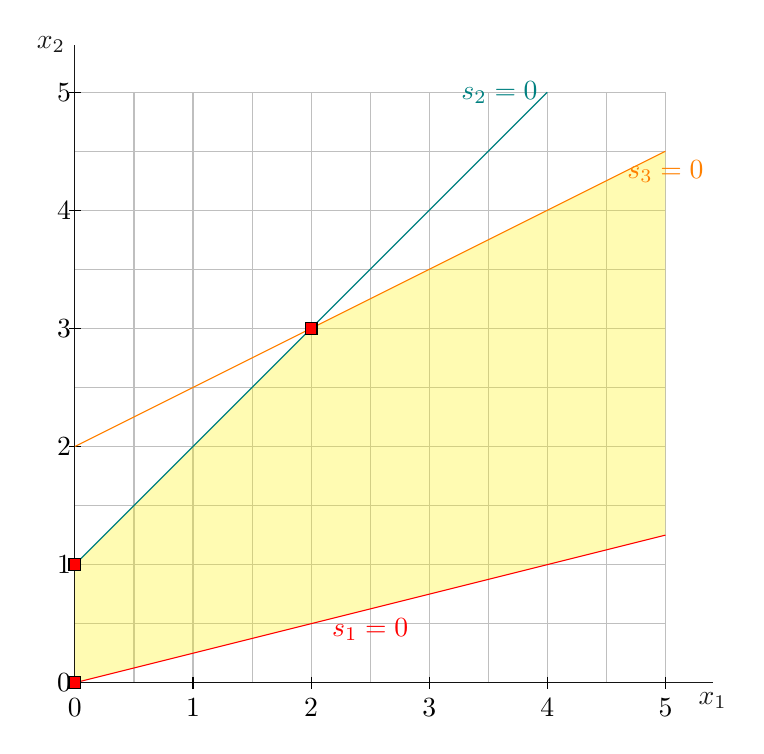
\begin{tikzpicture} [scale=1.5]
    \draw[gray!50, thin, step=.5] (0,0) grid (5,5);
    \draw[opacity=0.9] (0,0) -- (5.4,0) node[below] {$x_1$};
    \draw[opacity=0.9] (0,0) -- (0,5.4) node[left] {$x_2$}; % option \draw[very thick,->]

    \foreach \x in {0,...,5} \draw (\x,0.05) -- (\x,-0.05) node[below] {\x};
    \foreach \y in {0,...,5} \draw (-0.05,\y) -- (0.05,\y) node[left] {\y};

    \fill[yellow,opacity=0.3] (0,0) -- (0,1) -- (2,3) -- (5,4.5) --(5,1.25)-- cycle;

    \draw [red](0,0) -- node[below] {$s_1=0$} (5, 1.25);
    \draw [teal] (0,1)  --  (4,5) node[left, sloped] {$s_2=0$};
    \draw [orange](0,2) --  (5,4.5) node[below, sloped] {$s_3=0$}; %node[above right ,sloped] 
	\filldraw[fill=red] (-0.05,-0.05) rectangle (0.05,0.05);
	\filldraw[fill=red] (-0.05,.95) rectangle (0.05,1.05);
	\filldraw[fill=red] (1.95,2.95) rectangle (2.05,3.05);
\end{tikzpicture} \end{center} 
\end{minipage}

\begin{center}  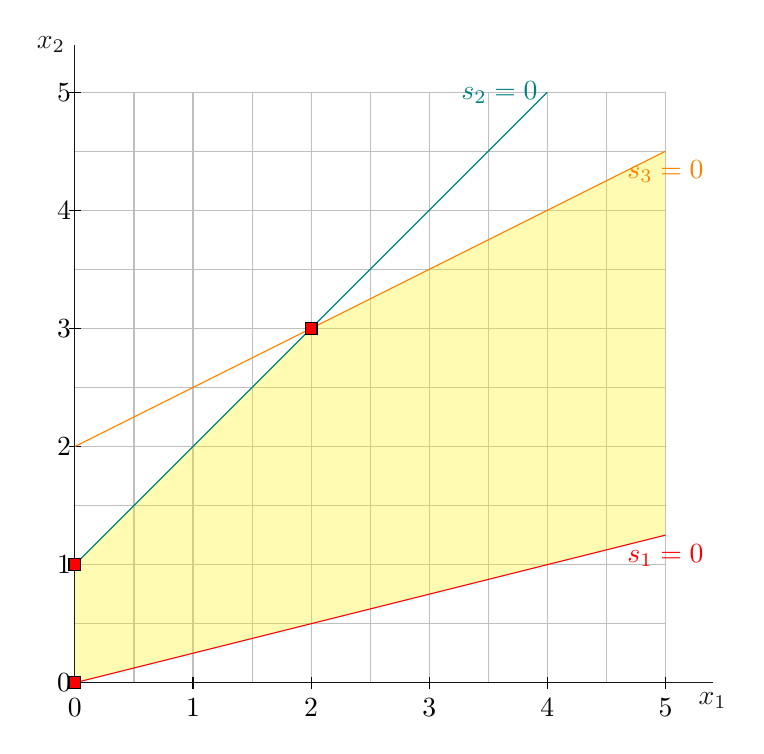
\begin{tikzpicture} [scale=1.5]
    \draw[gray!50, thin, step=.5] (0,0) grid (5,5);
    \draw[opacity=0.9] (0,0) -- (5.4,0) node[below] {$x_1$};
    \draw[opacity=0.9] (0,0) -- (0,5.4) node[left] {$x_2$}; % option \draw[very thick,->]

    \foreach \x in {0,...,5} \draw (\x,0.05) -- (\x,-0.05) node[below] {\x};
    \foreach \y in {0,...,5} \draw (-0.05,\y) -- (0.05,\y) node[left] {\y};

    \fill[yellow,opacity=0.3] (0,0) -- (0,1) -- (2,3) -- (5,4.5) --(5,1.25)-- cycle;

\draw[domain=0:4,smooth,variable=\x, teal] plot ({\x},{\x+1}) node[left] {$s_2=0$};
\draw[domain=0:5,smooth,variable=\x, red] plot ({\x},{\x*1/4}) node[below] {$s_1=0$};
%    \draw [red](0,0) -- node[below] {$s_1=0$} (5, 1.25);
    %\draw [teal] (0,1)  --  (4,5) node[left, sloped] {$s_2=0$};
    \draw [orange](0,2) --  (5,4.5) node[below, sloped] {$s_3=0$}; %node[above right ,sloped] 
	\filldraw[fill=red] (-0.05,-0.05) rectangle (0.05,0.05);
	\filldraw[fill=red] (-0.05,.95) rectangle (0.05,1.05);
	\filldraw[fill=red] (1.95,2.95) rectangle (2.05,3.05);
\end{tikzpicture} \end{center} 

% \draw[scale=0.5,domain=-3:3,smooth,variable=\x,blue] plot ({\x},{\x*\x});


  
\medskip E.g., consider the $s_3=0$ (orange) line, to find the extreme direction start at extreme point (2,3) and find another feasible point on the orange line, say (4,4) and subtract (2,3) from (4,4), which yields (2,1). 

\medskip This is related to the slope in two-dimensions, as discussed in class, the rise is 1 and the run is 2. So this direction has a slope of 1/2, but this does not carry over easily to higher dimensions where directions cannot be defined by a single number. 

\medskip To find the extreme directions we can change the right-hand-side to $\mathbf{b} = \mathbf{0}$, which forms a polyhedral cone (in yellow), and then add the constraint $x_1 + x_2 = 1$. The intersection of the cone and  $x_1 + x_2 = 1$ form a line segment.

\begin{minipage}[t][][b]{.4\linewidth} \vspace{0mm}
\begin{align*}
\mbox{max~~} & z = -5x_1 - x_2  \\
\mbox{s.t.~~} & x_1 - 4x_2 +s_1 = 0  \\
& -x_1 + x_2 + s_2 = 0 \\
& -x_1 + 2x_2 +s_3 = 0 \\
& x_1 + x_2 = 1 \\
& x_1, x_2, s_1, s_2, s_3 \ge 0.
\end{align*}
\end{minipage}%
\begin{minipage}[t][][b]{.6\linewidth}
\begin{center} 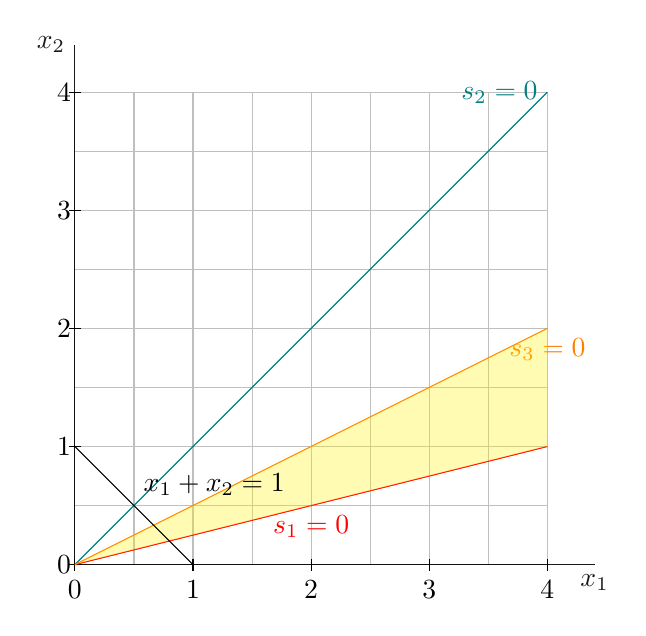
\begin{tikzpicture} [scale=1.5]
\draw[gray!50, thin, step=.5] (0,0) grid (4,4);
\draw[opacity=0.9] (0,0) -- (4.4,0) node[below] {$x_1$};
\draw[opacity=0.9] (0,0) -- (0,4.4) node[left] {$x_2$}; % option \draw[very thick,->]

\foreach \x in {0,...,4} \draw (\x,0.05) -- (\x,-0.05) node[below] {\x};
\foreach \y in {0,...,4} \draw (-0.05,\y) -- (0.05,\y) node[left] {\y};
        
\draw [red](0, 0) -- node[below] {$s_1=0$} (4, 1);
\draw [teal] (0,0)  -- (4,4) node[left, sloped] {$s_2=0$};
\draw [orange](0,0) -- (4,2) node[below, sloped] {$s_3=0$}; 
\fill[yellow,opacity=0.3] (0,0) -- (4,2) -- (4,1) --  cycle; % \draw [orange!50!blue] 

\draw [black] (0,1)  -- node[above right] {$x_1+x_2 = 1$} (1,0); 
\end{tikzpicture} \end{center} 
\end{minipage}



\begin{center} 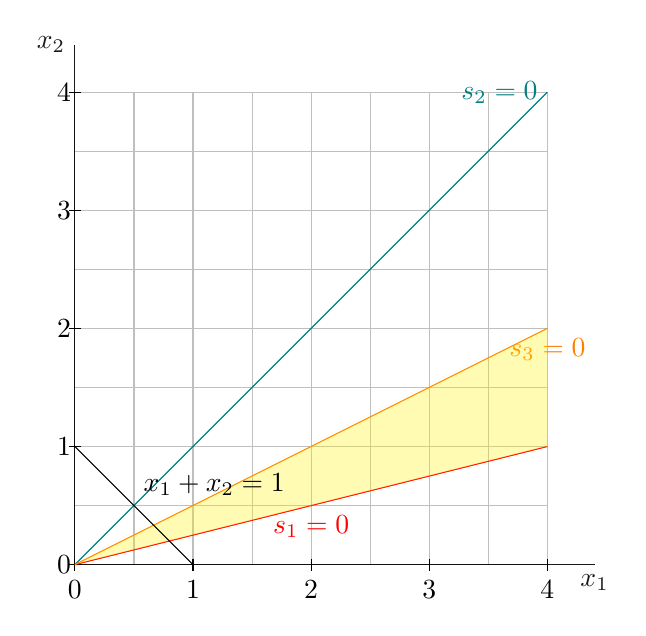
\begin{tikzpicture} [scale=1.5]
\draw[gray!50, thin, step=.5] (0,0) grid (4,4);
\draw[opacity=0.9] (0,0) -- (4.4,0) node[below] {$x_1$};
\draw[opacity=0.9] (0,0) -- (0,4.4) node[left] {$x_2$}; % option \draw[very thick,->]

\foreach \x in {0,...,4} \draw (\x,0.05) -- (\x,-0.05) node[below] {\x};
\foreach \y in {0,...,4} \draw (-0.05,\y) -- (0.05,\y) node[left] {\y};
        
\draw [red](0, 0) -- node[below] {$s_1=0$} (4, 1);
\draw [teal] (0,0)  -- (4,4) node[left, sloped] {$s_2=0$};
\draw [orange](0,0) -- (4,2) node[below, sloped] {$s_3=0$}; 
\fill[yellow,opacity=0.3] (0,0) -- (4,2) -- (4,1) --  cycle; % \draw [orange!50!blue] 

\draw [black] (0,1)  -- node[above right] {$x_1+x_2 = 1$} (1,0); 
\end{tikzpicture} \end{center} 


\medskip Magnifying for clarity, and removing the $s_2=0$ (teal) line, as it is redundant, and marking the extreme points of the new feasible region, (4/5, 1/5) and (2/3, 1/3), with red boxes, we have:

\begin{center}  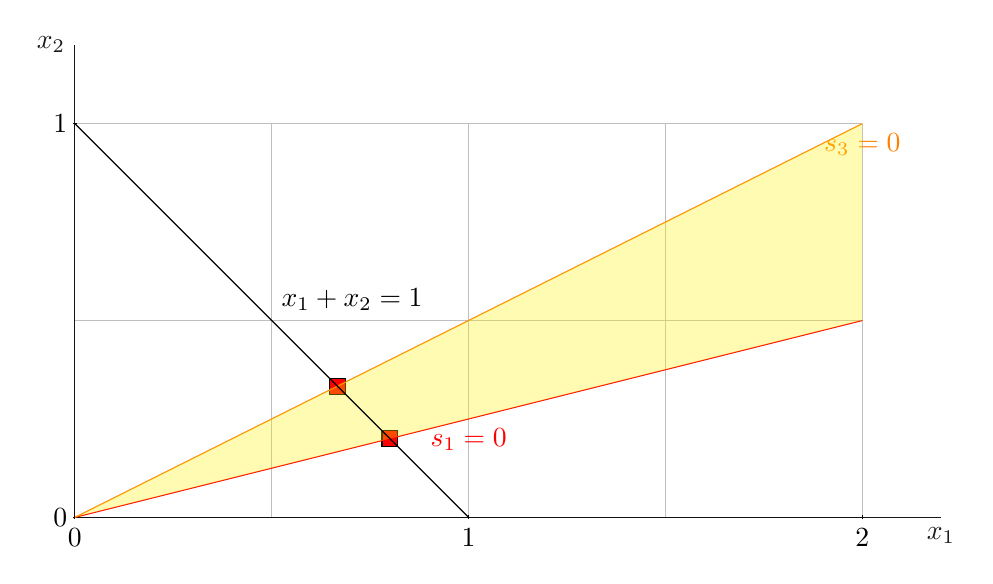
\begin{tikzpicture} [x=50mm, y=50mm] [scale=1.5]
\draw[gray!50, thin, step=.5] (0,0) grid (2,1);
\draw[opacity=0.9] (0,0) -- (2.2,0) node[below] {$x_1$};
\draw[opacity=0.9] (0,0) -- (0,1.2) node[left] {$x_2$}; % option \draw[very thick,->]

\foreach \x in {0,...,2} \draw (\x,0.005) -- (\x,-0.005) node[below] {\x};
\foreach \y in {0,...,1} \draw (-0.005,\y) -- (0.005,\y) node[left] {\y};

\filldraw[fill=red] (0.8-0.02,0.2-0.02) rectangle (0.8+0.02,0.2+0.02);
\filldraw[fill=red] (0.667-0.02,0.333-0.02) rectangle (0.667+0.02,0.333+0.02);

\draw [red](0, 0) -- node[below] {$s_1=0$} (2, .5);
\draw [orange](0,0) -- (2,1) node[below, sloped] {$s_3=0$}; 
\fill[yellow,opacity=0.3] (0,0) -- (2,.5) -- (2,1) --  cycle; % \draw [orange!50!blue] 
\draw [black] (0,1)  -- node[above right] {$x_1+x_2 = 1$} (1,0); 
\end{tikzpicture} \end{center} 

The extreme directions are thus (4/5, 1/5) and (2/3, 1/3). \\

{\bf Representation Theorem:} Let  $\mathbf{x_1}, \mathbf{x_2},\cdots \mathbf{x_k}$ be the set of extreme points of $\mathcal{S}$, and if $\mathcal{S}$ is unbounded, $\mathbf{d_1}, \mathbf{d_2},\cdots \mathbf{d_l}$ be the set of extreme directions. Then any $\mathbf{x} \in \mathcal{S}$ is equal to a convex combination of the extreme points and a non-negative linear combination of the extreme directions: $\mathbf{x} = \sum_{j=1}^k \lambda_j \mathbf{x_j} + \sum_{j=1}^l \mu_j \mathbf{d_j}$, where $\sum_{j=1}^k \lambda_j = 1$, $\lambda_j \ge 0,~\forall  j=1,2,\cdots,k$, and $\mu_j \ge 0,~\forall j=1,2,\cdots,l$.

 \begin{minipage}[t][][b]{.4\linewidth}
\begin{align*}
\mbox{max~~} & z = -5x_1 - x_2  \\\
\mbox{s.t.~~} & x_1 - 4x_2 +s_1 = 0  \\
& -x_1 + x_2 + s_2 = 1 \\
& -x_1 + 2x_2 +s_3 = 4 \\
& x_1, x_2, s_1, s_2, s_3 \ge 0.
\end{align*}
\end{minipage}%
\begin{minipage}[t][][b]{.6\linewidth}
\begin{center}  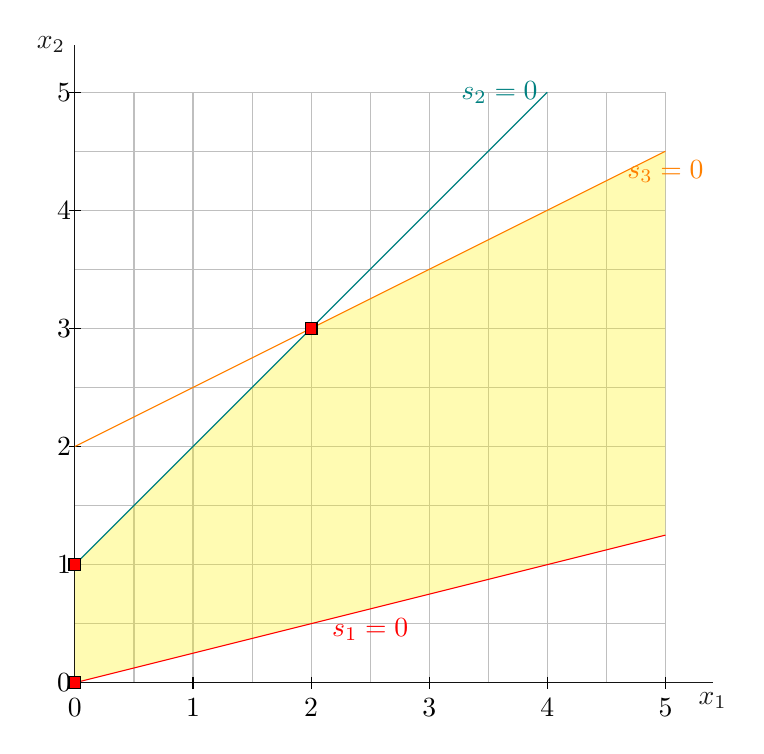
\begin{tikzpicture} [scale=1.5]
    \draw[gray!50, thin, step=.5] (0,0) grid (5,5);
    \draw[opacity=0.9] (0,0) -- (5.4,0) node[below] {$x_1$};
    \draw[opacity=0.9] (0,0) -- (0,5.4) node[left] {$x_2$}; % option \draw[very thick,->]

    \foreach \x in {0,...,5} \draw (\x,0.05) -- (\x,-0.05) node[below] {\x};
    \foreach \y in {0,...,5} \draw (-0.05,\y) -- (0.05,\y) node[left] {\y};

    \fill[yellow,opacity=0.3] (0,0) -- (0,1) -- (2,3) -- (5,4.5) --(5,1.25)-- cycle;

    \draw [red](0,0) -- node[below] {$s_1=0$} (5, 1.25);
    \draw [teal] (0,1)  --  (4,5) node[left, sloped] {$s_2=0$};
    \draw [orange](0,2) --  (5,4.5) node[below, sloped] {$s_3=0$}; %node[above right ,sloped] 
	\filldraw[fill=red] (-0.05,-0.05) rectangle (0.05,0.05);
	\filldraw[fill=red] (-0.05,.95) rectangle (0.05,1.05);
	\filldraw[fill=red] (1.95,2.95) rectangle (2.05,3.05);
\end{tikzpicture} \end{center} 
\end{minipage}




Represent point (1/2, 1) as a convex combination of the extreme points of the above LP.  Find $\lambda$s to solve the following system of equations:

$$\lambda_1 \left[
  \begin{array}{c}
  0 \\
  0 \\
  \end{array} \right]+
 \lambda_2 \left[
  \begin{array}{c}
  0 \\
  1 \\
  \end{array} \right] +
 \lambda_3 \left[
  \begin{array}{c}
  2 \\
  3 \\
  \end{array} \right]  =
 \left[
  \begin{array}{c}
  1/2 \\
  1 \\
  \end{array} \right] 
$$


\newpage The Variable (Canonical Form) and Requirement Space 

\begin{minipage}[t][][b]{.4\linewidth}
\begin{align*}
\mbox{max~~} & z = 2x_1 + x_2  \\\
\mbox{s.t.~~} & x_1 - x_2 +s_1 =  2  \\
& x_1 + x_2 +s_2  = 3 \\
& x_1, x_2, s_1 , s_2  \ge 0.
\end{align*}
\end{minipage}%
\begin{minipage}[t][][b]{.6\linewidth}
\begin{center}  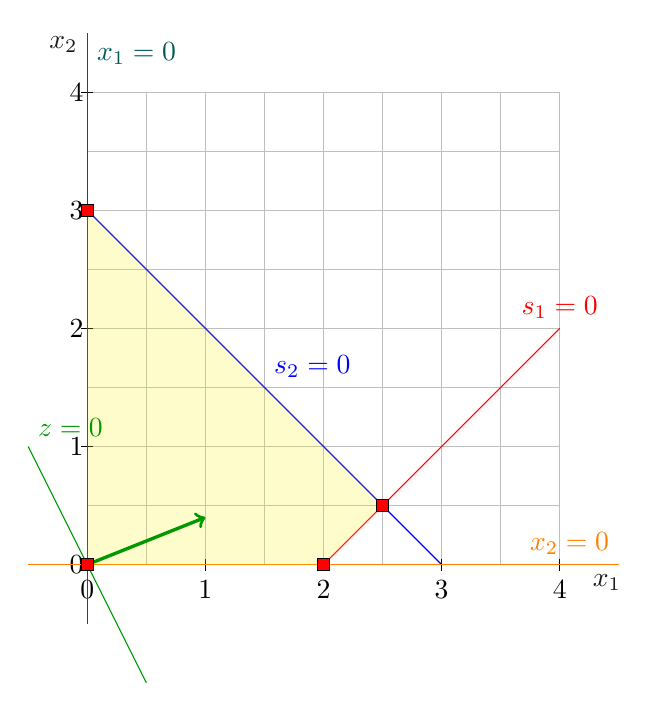
\begin{tikzpicture} [scale=1.5]
\draw[gray!50, thin, step=.5] (0,0) grid (4,4);
\draw[opacity=0.9] (0,0) -- (4.4,0) node[below] {$x_1$};
\draw[opacity=0.9] (0,0) -- (0,4.4) node[left] {$x_2$};

\foreach \x in {0,...,4} \draw (\x,0.05) -- (\x,-0.05) node[below] {\x};
\foreach \y in {0,...,4} \draw (-0.05,\y) -- (0.05,\y) node[left] {\y};

\draw [red](2, 0) --  (4, 2) node[above] {$s_1= 0$};
\draw [blue] (0,3)  -- node[above right] {$s_2=0$} (3,0) ;
\draw [teal!70!black](0,-.5) --  (0,4.5) node[below right] {$x_1=0$}; 
\draw [orange](-.5,0) --  (4.5,0) node[above left] {$x_2=0$}; 

\fill[yellow,opacity=0.2] (0,0) -- (2,0) -- (2.5,0.5) -- (0,3) -- cycle;

\draw [green!60!black] (-0.5, 1)  node[above right] {$z=0$} --  (0.5, -1)  ; % o.f.
\draw [green!60!black, very thick,->](0,0) -- (0+1, 0+2/5); % gradient

\filldraw[fill=red] (-0.05,-0.05) rectangle (0.05,0.05);
\filldraw[fill=red] (2.45,0.45) rectangle (2.55,0.55);
\filldraw[fill=red] (1.95,-0.05) rectangle (2.05,0.05);
\filldraw[fill=red] (-0.05,2.95) rectangle (0.05,3.05);    
\end{tikzpicture} \end{center} 
\end{minipage}



\begin{minipage}[t][][b]{.4\linewidth}
\begin{align*}
\mbox{max~~} & z = 2x_1 + x_2  \\\
\mbox{s.t.~~} & x_1 - x_2 +s_1 =  2  \\
& x_1 + x_2 +s_2  = 3 \\
& x_1, x_2, s_1 , s_2  \ge 0.
\end{align*}
\end{minipage}%
\begin{minipage}[t][][b]{.6\linewidth}
\begin{center}  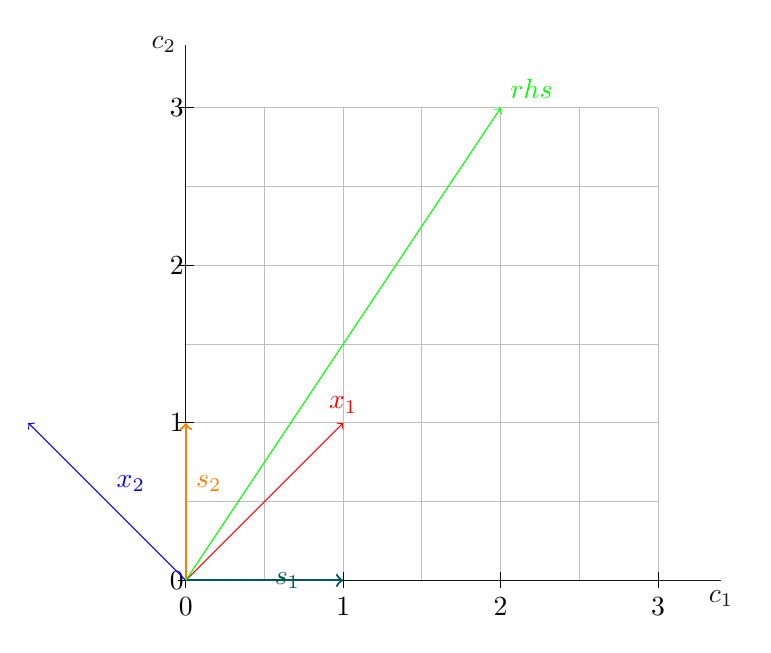
\begin{tikzpicture}[x=20mm, y=20mm] [scale=1.5]  % requirement space
\draw[gray!50, thin, step=.5] (0,0) grid (3,3);
\draw[opacity=0.9] (0,0) -- (3.4,0) node[below] {$c_1$};
\draw[opacity=0.9] (0,0) -- (0,3.4) node[left] {$c_2$};

\foreach \x in {0,...,3} \draw (\x,0.05) -- (\x,-0.05) node[below] {\x};
\foreach \y in {0,...,3} \draw (-0.05,\y) -- (0.05,\y) node[left] {\y};

\draw [red,->](0, 0) --  (1, 1) node[above] {$x_1$};
\draw [blue,->] (0,0)  -- node[above right] {$x_2$} (-1,1) ;
\draw [thick, teal!70!black,->](0,0) -- node[right] {$s_1$} (1,0); 
\draw [thick, orange,->](0,0) -- node[above right] {$s_2$} (0,1); 
\draw [green,->] (0, 0)  --  (2,3) node[above right] {$rhs$}   ; 
\end{tikzpicture} \end{center} 
\end{minipage}
